%% bare_conf.tex
%% V1.4b
%% 2015/08/26
%% by Michael Shell
%% See:
%% http://www.michaelshell.org/
%% for current contact information.
%%
%% This is a skeleton file demonstrating the use of IEEEtran.cls
%% (requires IEEEtran.cls version 1.8b or later) with an IEEE
%% conference paper.
%%
%% Support sites:
%% http://www.michaelshell.org/tex/ieeetran/
%% http://www.ctan.org/pkg/ieeetran
%% and
%% http://www.ieee.org/

%%*************************************************************************
%% Legal Notice:
%% This code is offered as-is without any warranty either expressed or
%% implied; without even the implied warranty of MERCHANTABILITY or
%% FITNESS FOR A PARTICULAR PURPOSE! 
%% User assumes all risk.
%% In no event shall the IEEE or any contributor to this code be liable for
%% any damages or losses, including, but not limited to, incidental,
%% consequential, or any other damages, resulting from the use or misuse
%% of any information contained here.
%%
%% All comments are the opinions of their respective authors and are not
%% necessarily endorsed by the IEEE.
%%
%% This work is distributed under the LaTeX Project Public License (LPPL)
%% ( http://www.latex-project.org/ ) version 1.3, and may be freely used,
%% distributed and modified. A copy of the LPPL, version 1.3, is included
%% in the base LaTeX documentation of all distributions of LaTeX released
%% 2003/12/01 or later.
%% Retain all contribution notices and credits.
%% ** Modified files should be clearly indicated as such, including  **
%% ** renaming them and changing author support contact information. **
%%*************************************************************************


% *** Authors should verify (and, if needed, correct) their LaTeX system  ***
% *** with the testflow diagnostic prior to trusting their LaTeX platform ***
% *** with production work. The IEEE's font choices and paper sizes can   ***
% *** trigger bugs that do not appear when using other class files.       ***                          ***
% The testflow support page is at:
% http://www.michaelshell.org/tex/testflow/



\documentclass[conference]{IEEEtran}
% Some Computer Society conferences also require the compsoc mode option,
% but others use the standard conference format.
%
% If IEEEtran.cls has not been installed into the LaTeX system files,
% manually specify the path to it like:
% \documentclass[conference]{../sty/IEEEtran}





% Some very useful LaTeX packages include:
% (uncomment the ones you want to load)


% *** MISC UTILITY PACKAGES ***
%
%\usepackage{ifpdf}
% Heiko Oberdiek's ifpdf.sty is very useful if you need conditional
% compilation based on whether the output is pdf or dvi.
% usage:
% \ifpdf
%   % pdf code
% \else
%   % dvi code
% \fi
% The latest version of ifpdf.sty can be obtained from:
% http://www.ctan.org/pkg/ifpdf
% Also, note that IEEEtran.cls V1.7 and later provides a builtin
% \ifCLASSINFOpdf conditional that works the same way.
% When switching from latex to pdflatex and vice-versa, the compiler may
% have to be run twice to clear warning/error messages.


% *** CITATION PACKAGES ***
%
\usepackage{cite}
% cite.sty was written by Donald Arseneau
% V1.6 and later of IEEEtran pre-defines the format of the cite.sty package
% \cite{} output to follow that of the IEEE. Loading the cite package will
% result in citation numbers being automatically sorted and properly
% "compressed/ranged". e.g., [1], [9], [2], [7], [5], [6] without using
% cite.sty will become [1], [2], [5]--[7], [9] using cite.sty. cite.sty's
% \cite will automatically add leading space, if needed. Use cite.sty's
% noadjust option (cite.sty V3.8 and later) if you want to turn this off
% such as if a citation ever needs to be enclosed in parenthesis.
% cite.sty is already installed on most LaTeX systems. Be sure and use
% version 5.0 (2009-03-20) and later if using hyperref.sty.
% The latest version can be obtained at:
% http://www.ctan.org/pkg/cite
% The documentation is contained in the cite.sty file itself.


% *** GRAPHICS RELATED PACKAGES ***
%
\ifCLASSINFOpdf
\usepackage[pdftex]{graphicx}
  % declare the path(s) where your graphic files are
  % \graphicspath{{../pdf/}{../jpeg/}}
  % and their extensions so you won't have to specify these with
  % every instance of \includegraphics
  % \DeclareGraphicsExtensions{.pdf,.jpeg,.png}
\else
  % or other class option (dvipsone, dvipdf, if not using dvips). graphicx
  % will default to the driver specified in the system graphics.cfg if no
  % driver is specified.
  % \usepackage[dvips]{graphicx}
  % declare the path(s) where your graphic files are
  % \graphicspath{{../eps/}}
  % and their extensions so you won't have to specify these with
  % every instance of \includegraphics
  % \DeclareGraphicsExtensions{.eps}
\fi
% graphicx was written by David Carlisle and Sebastian Rahtz. It is
% required if you want graphics, photos, etc. graphicx.sty is already
% installed on most LaTeX systems. The latest version and documentation
% can be obtained at: 
% http://www.ctan.org/pkg/graphicx
% Another good source of documentation is "Using Imported Graphics in
% LaTeX2e" by Keith Reckdahl which can be found at:
% http://www.ctan.org/pkg/epslatex
%
% latex, and pdflatex in dvi mode, support graphics in encapsulated
% postscript (.eps) format. pdflatex in pdf mode supports graphics
% in .pdf, .jpeg, .png and .mps (metapost) formats. Users should ensure
% that all non-photo figures use a vector format (.eps, .pdf, .mps) and
% not a bitmapped formats (.jpeg, .png). The IEEE frowns on bitmapped formats
% which can result in "jaggedy"/blurry rendering of lines and letters as
% well as large increases in file sizes.
%
% You can find documentation about the pdfTeX application at:
% http://www.tug.org/applications/pdftex

% *** MATH PACKAGES ***
%
%\usepackage{amsmath}
% A popular package from the American Mathematical Society that provides
% many useful and powerful commands for dealing with mathematics.
%
% Note that the amsmath package sets \interdisplaylinepenalty to 10000
% thus preventing page breaks from occurring within multiline equations. Use:
%\interdisplaylinepenalty=2500
% after loading amsmath to restore such page breaks as IEEEtran.cls normally
% does. amsmath.sty is already installed on most LaTeX systems. The latest
% version and documentation can be obtained at:
% http://www.ctan.org/pkg/amsmath

% *** SPECIALIZED LIST PACKAGES ***
%
\usepackage{algorithm}
\usepackage{algpseudocode}
% algorithmic.sty was written by Peter Williams and Rogerio Brito.
% This package provides an algorithmic environment fo describing algorithms.
% You can use the algorithmic environment in-text or within a figure
% environment to provide for a floating algorithm. Do NOT use the algorithm
% floating environment provided by algorithm.sty (by the same authors) or
% algorithm2e.sty (by Christophe Fiorio) as the IEEE does not use dedicated
% algorithm float types and packages that provide these will not provide
% correct IEEE style captions. The latest version and documentation of
% algorithmic.sty can be obtained at:
% http://www.ctan.org/pkg/algorithms
% Also of interest may be the (relatively newer and more customizable)
% algorithmicx.sty package by Szasz Janos:
% http://www.ctan.org/pkg/algorithmicx

% *** ALIGNMENT PACKAGES ***
%
%\usepackage{array}
% Frank Mittelbach's and David Carlisle's array.sty patches and improves
% the standard LaTeX2e array and tabular environments to provide better
% appearance and additional user controls. As the default LaTeX2e table
% generation code is lacking to the point of almost being broken with
% respect to the quality of the end results, all users are strongly
% advised to use an enhanced (at the very least that provided by array.sty)
% set of table tools. array.sty is already installed on most systems. The
% latest version and documentation can be obtained at:
% http://www.ctan.org/pkg/array


% IEEEtran contains the IEEEeqnarray family of commands that can be used to
% generate multiline equations as well as matrices, tables, etc., of high
% quality.


% *** SUBFIGURE PACKAGES ***
%\ifCLASSOPTIONcompsoc
%  \usepackage[caption=false,font=normalsize,labelfont=sf,textfont=sf]{subfig}
%\else
%  \usepackage[caption=false,font=footnotesize]{subfig}
%\fi
% subfig.sty, written by Steven Douglas Cochran, is the modern replacement
% for subfigure.sty, the latter of which is no longer maintained and is
% incompatible with some LaTeX packages including fixltx2e. However,
% subfig.sty requires and automatically loads Axel Sommerfeldt's caption.sty
% which will override IEEEtran.cls' handling of captions and this will result
% in non-IEEE style figure/table captions. To prevent this problem, be sure
% and invoke subfig.sty's "caption=false" package option (available since
% subfig.sty version 1.3, 2005/06/28) as this is will preserve IEEEtran.cls
% handling of captions.
% Note that the Computer Society format requires a larger sans serif font
% than the serif footnote size font used in traditional IEEE formatting
% and thus the need to invoke different subfig.sty package options depending
% on whether compsoc mode has been enabled.
%
% The latest version and documentation of subfig.sty can be obtained at:
% http://www.ctan.org/pkg/subfig




% *** FLOAT PACKAGES ***
%
%\usepackage{fixltx2e}
% fixltx2e, the successor to the earlier fix2col.sty, was written by
% Frank Mittelbach and David Carlisle. This package corrects a few problems
% in the LaTeX2e kernel, the most notable of which is that in current
% LaTeX2e releases, the ordering of single and double column floats is not
% guaranteed to be preserved. Thus, an unpatched LaTeX2e can allow a
% single column figure to be placed prior to an earlier double column
% figure.
% Be aware that LaTeX2e kernels dated 2015 and later have fixltx2e.sty's
% corrections already built into the system in which case a warning will
% be issued if an attempt is made to load fixltx2e.sty as it is no longer
% needed.
% The latest version and documentation can be found at:
% http://www.ctan.org/pkg/fixltx2e


%\usepackage{stfloats}
% stfloats.sty was written by Sigitas Tolusis. This package gives LaTeX2e
% the ability to do double column floats at the bottom of the page as well
% as the top. (e.g., "\begin{figure*}[!b]" is not normally possible in
% LaTeX2e). It also provides a command:
%\fnbelowfloat
% to enable the placement of footnotes below bottom floats (the standard
% LaTeX2e kernel puts them above bottom floats). This is an invasive package
% which rewrites many portions of the LaTeX2e float routines. It may not work
% with other packages that modify the LaTeX2e float routines. The latest
% version and documentation can be obtained at:
% http://www.ctan.org/pkg/stfloats
% Do not use the stfloats baselinefloat ability as the IEEE does not allow
% \baselineskip to stretch. Authors submitting work to the IEEE should note
% that the IEEE rarely uses double column equations and that authors should try
% to avoid such use. Do not be tempted to use the cuted.sty or midfloat.sty
% packages (also by Sigitas Tolusis) as the IEEE does not format its papers in
% such ways.
% Do not attempt to use stfloats with fixltx2e as they are incompatible.
% Instead, use Morten Hogholm'a dblfloatfix which combines the features
% of both fixltx2e and stfloats:
%
% \usepackage{dblfloatfix}
% The latest version can be found at:
% http://www.ctan.org/pkg/dblfloatfix

% *** PDF, URL AND HYPERLINK PACKAGES ***
%
\usepackage{url}
% url.sty was written by Donald Arseneau. It provides better support for
% handling and breaking URLs. url.sty is already installed on most LaTeX
% systems. The latest version and documentation can be obtained at:
% http://www.ctan.org/pkg/url
% Basically, \url{my_url_here}.




% *** Do not adjust lengths that control margins, column widths, etc. ***
% *** Do not use packages that alter fonts (such as pslatex).         ***
% There should be no need to do such things with IEEEtran.cls V1.6 and later.
% (Unless specifically asked to do so by the journal or conference you plan
% to submit to, of course. )


% correct bad hyphenation here
\hyphenation{op-tical net-works semi-conduc-tor}


\begin{document}
%
% paper title
% Titles are generally capitalized except for words such as a, an, and, as,
% at, but, by, for, in, nor, of, on, or, the, to and up, which are usually
% not capitalized unless they are the first or last word of the title.
% Linebreaks \\ can be used within to get better formatting as desired.
% Do not put math or special symbols in the title.
\title{Rapid detection of disobedient forwarding on a compromised OpenFlow switch}


% author names and affiliations
% use a multiple column layout for up to three different
% affiliations
\author{\IEEEauthorblockN{Yen-Chun Chiu, Po-Ching Lin}
\IEEEauthorblockA{Department of Computer Science and\\Information Engineering\\
National Chung Cheng University\\
Chiayi, Taiwan 62102\\
Email: shuaichiou@gmail.com, pclin@cs.ccu.edu.tw}}

% conference papers do not typically use \thanks and this command
% is locked out in conference mode. If really needed, such as for
% the acknowledgment of grants, issue a \IEEEoverridecommandlockouts
% after \documentclass

% for over three affiliations, or if they all won't fit within the width
% of the page, use this alternative format:
% 
%\author{\IEEEauthorblockN{Michael Shell\IEEEauthorrefmark{1},
%Homer Simpson\IEEEauthorrefmark{2},
%James Kirk\IEEEauthorrefmark{3}, 
%Montgomery Scott\IEEEauthorrefmark{3} and
%Eldon Tyrell\IEEEauthorrefmark{4}}
%\IEEEauthorblockA{\IEEEauthorrefmark{1}School of Electrical and Computer Engineering\\
%Georgia Institute of Technology,
%Atlanta, Georgia 30332--0250\\ Email: see http://www.michaelshell.org/contact.html}
%\IEEEauthorblockA{\IEEEauthorrefmark{2}Twentieth Century Fox, Springfield, USA\\
%Email: homer@thesimpsons.com}
%\IEEEauthorblockA{\IEEEauthorrefmark{3}Starfleet Academy, San Francisco, California 96678-2391\\
%Telephone: (800) 555--1212, Fax: (888) 555--1212}
%\IEEEauthorblockA{\IEEEauthorrefmark{4}Tyrell Inc., 123 Replicant Street, Los Angeles, California 90210--4321}}

% use for special paper notices
%\IEEEspecialpapernotice{(Invited Paper)}

% make the title area
\maketitle

% As a general rule, do not put math, special symbols or citations
% in the abstract
\begin{abstract}
Software-defined networking (SDN) is programmable, centrally managed, and flexible with topology alteration. It allows network administrators to manage network flows easily from a centralized controller. However, these new features also lead to new security threats with applications, controllers, OpenFlow switches, topology management and so on. In this work, we study the attack of compromising a switch, and design a method to detect disobedient forwarding in the flow table. To enhance the detection efficiency and minimize additional network traffic, we reduce the number of detection packets necessary by aggregating the flow entries in a short time. To aggregate the flow entries, we select entries whose match fields are able to compose a valid packet from different switches. The switches on which the entries are form a path that allows the packet to travel through for rapid detection. We evaluate the effectiveness of this detection method in various topology types typically found in a data center network by Mininet simulation. The experimental result demonstrates that this method can examine the forwarding correctness of nearly 3 flow entries simultaneously on average for each detection packet. Furthermore, since the positive and negative factors to the growth of aggregation rates break even in a large topology, the scale of the network topology does not affect the efficiency of the method significantly.
\end{abstract}

% no keywords
% For peer review papers, you can put extra information on the cover
% page as needed:
% \ifCLASSOPTIONpeerreview
% \begin{center} \bfseries EDICS Category: 3-BBND \end{center}
% \fi
%
% For peerreview papers, this IEEEtran command inserts a page break and
% creates the second title. It will be ignored for other modes.
\IEEEpeerreviewmaketitle

\section{Introduction}
\label{chap:intro}
Software-defined networking (SDN) is a dynamic, programmable, cost-effective solution that gains great popularity in the industry and academia in recent years. A controller can centrally manage the flow rules on the switches in a consistent manner, and network applications can be developed on the controller for flexible management. Nevertheless, SDN often comes with new security threats \cite{SOS13} as new mechanisms such as topology discovery, host management, OpenFlow protocols and application interfaces have been introduced. For example, applications may be malicious, topology discovery and host management mechanisms can be leveraged to launch man-in-the-middle or denial-of-service attacks, malicious controllers may affect the control channel, and switches and hosts may be compromised.

Since Openflow switches lie between the controller and the hosts, an attacker can utilize a number of components to perform attacks. In \cite{HXWG15}, Hong et al. studied the attacks that poison network visibility and its countermeasure, but the situation in which switches are compromised is not considered. Also, a compromised switch is able to modify its own flow entries for malicious behavior like undesired forwarding or packet dropping. It can also connect to a malicious controller and influence the network by manipulating the control traffic in the way the attacker desires, such as sending forged OpenFlow messages. Another type of attack is to exploit the topology discovery mechanism, making the controller into believing the existence of non-existing links.

Although some protection methods have been proposed \cite{CKGL15,PJL16}, there has not been an efficient way to detect if there is any compromised switch in SDN. The detection method in \cite{CKGL15} is able to detect whether a flow entry works as expected. However, it tests only one flow entry at a time, which is inefficient in a large network. FADE presented in \cite{PJL16} results in some false negative results and takes a while to go through the entire network. ATPG in \cite{ZKVM12} is able to test through all the rules in the network with few packets in a short time. However, it is designed for regular networks in the Internet, deployment takes a lot of efforts such as setting up test terminals and network monitors. In this work, we present a method to discover compromised switches if they do not follow the flow rules, it reduces the cost of detecting compromised switches and speed up the entire detection process flexibly. We fabricate the detection packets so that each can test multiple flow entries on multiple switches at a time by exploiting identical match field values or exclusive match fields in the flow entries. 
The main contributions of this work are as follows:

\begin{enumerate}
\item
Analyze attacks related to flow entry manipulation, which influences the visibility of network.
\item
Discuss existing countermeasures to such attacks.
\item
Propose a switch entry validation method that verifies all the entries inside the network with aggregation technique.
\item
Evaluate the effectiveness of the method with various control variables.
\end{enumerate}

The following chapters in this work are organized as follows. Section 2 gives detailed background knowledge of related technology and discusses possible threats and countermeasures. Section 3 is about the threat model and the theory behind the detection method. Section 4 contains the experimental details including setup, considerations and evaluation methods. Finally, the conclusion and future expectation of this work will be in Section 5.

\section{Background and related work}
\subsection{SDN and OpenFlow}
\label{SDN and OpenFlow}
OpenFlow is the most popular southbound interface in SDN, it maintains the abstract view of the network, including network topology, host positions and the states of network resources. A switch that supports OpenFlow is called an OpenFlow switch. OpenFlow switches typically separate OpenFlow and non-OpenFlow traffic, which do not interfere with each other. There is usually a table-miss entry with the lowest priority and wildcards in all the match fields, it is for handling the packets that cannot match any other flow entries. Normally, such a packet will be sent to the controller using the controller-reserved port, and the controller will decide how to process it and add a new flow entry according to the network policy. 

\subsection{Compromised OpenFlow switches}
\label{SDN security}
We will focus on the issue of compromised OpenFlow switches, since it has been less addressed than the others so far. Compromising OpenFlow switches can lead to some negative results: (1) Attackers may launch topology poisoning attack by manipulating link discovery packets. (2) The the flow entries on a compromised switch can be unexpectedly altered. (3) The packets that pass through a compromised switch can be eavesdropped or dropped. (4) The compromised switch may be configured to be managed by another malicious controller. (5) It is possible to launch network-wide denial-of-service attack by sending specific forged packets to consume the controller's resource. 

\subsubsection{Unwanted flow entry modification}
Unwanted flow entry modification on the compromised switch may lead to MITM, eavesdropping or DOS attack \cite{AAS14}. The detection method proposed in \cite{CKGL15} is able to detect whether a switch is forwarding the packets in an unexpected way. After selecting a flow entry as the detecting target, they install new entries on its neighbors. With the match field selected by their algorithm, they are able to let every packet that matches the new flow entry matches the target flow entry. A packet containing the match field of the new flow entry will be sent from \texttt{Packet\_Out} to a neighbor of the target switch, forwarded to the target switch, go through the series of switches, and should be sent back to the controller. Finally, they will check if the packet comes back to the controller as expected and remains unchanged. However, this method will take a long time to run if it is desired to scan through a large number of flow entries. A pre-detection method to narrow down the potential targets is needed.

In \cite{PJL16}, Pang et al. discuss about forwarding anomaly and design a method to detect the problem. First, they find a minimal set of flows whose rule paths cover all flows. Next, additional dedicated flow entries with timeout will be installed, the actions of these dedicated entries will modify the label, and a label will be added into packets to collect flow statistics. The more dedicated entries are used, the more likely they are able to identify where the malicious flow entry is located. However, if the dedicated rules are installed right on the malicious switch, the newly installed entry may be matched prior to the malicious entry and the method will not work. Therefore, they need to calculate the optimal number of dedicated entries to install to reach a balance between efficiency and probability to detect the malicious flow entries successfully. Their experimental result shows that FADE is able to detect forwarding anomaly in a network topology containing around 30 switches in 15 minutes with 2.5\% false negative and 4\% throughput reduction.

\subsubsection{Network debugging in SDN}
Some network debugging methods can be quite inspiring for the development of malicious behavior detection method. Flow entry information gathering techniques can also be found in \cite{ARDC14}. Just like traceroute, Agarwal et al. aim to trace the traveling path of a packet in an SDN network with minimal influence to the network. They use the VLAN field as color labels of switches. By setting up entries with color as match field in the way specified in \cite{ARDC14}, they are able to match the incoming probing packets from other switches and send them to the controller for logging, while not matching the probing packets from the controller and use the actual forwarding rules in the switch. Normally, the probing procedure repeats until the packet is consumed by a host or meets a loop. However, when malicious behavior like packet dropping occurs, it is also likely to find the culprit by checking the last hop of the probing packet.

Automatic Test Packet Generation (ATPG) proposed in \cite{ZKVM12} is able to test through tremendous number of flow rules and links with the packets less than 1\% of the traffic in an automatic way. They use ``rules'' to define how packets should be processed, and keep a list of rule histories for each pair of ingress and egress port. Similar to \cite{PJL16}, they find the minimal subset of test packets whose travel path covers the detection objective (entries, links or router queues), and check the packets to see if the actions are executed normally when it reach an end point. Since that work runs on regular networks, it requires deployment of terminals for generating test packets. In contrast, we utilize the trait of action set in OpenFlow and deploy new flow entries that are able to duplicate detection packets from a switch and send them to other switches in a tree-like manner. This increases the number of entries a single detection packet is able to detect. 

\section{Detection Algorithm}
This work focuses on the problem that a compromised switch will bring and presents the method to detect such a switch. Our method emphasizes on scanning through the whole network with fewer packets and high detection efficiency. In this chapter, we will define the threat models and how the problems can be solved with the presented detection algorithm.

\subsection{Threat models and Attack scenarios}
In this work, we assume the following scenarios of compromising a switch in the threat models:
\begin{enumerate}
\item
Only one OpenFlow switch is compromised. No cooperation among multiple compromised switches for attacks will happen.
\item
Other parts of the network such as the controller, other switches and hosts function normally. Any potential flaw is unintentional and out of the scope of this work.
\item
An attacker cannot totally change the way of switch processing or core mechanism, but only perform the attack by modifying flow entries.
\item
Initially, the network is clean, and nothing is compromised. The attacks take place some time after the whole network is established.
\end{enumerate}

\subsection{Rapid detection method of disobedient forwarding}
Our method aims to detect if the flow entries of switches in the network work as expected. It is inspired by \cite{CKGL15}. The method in this work has two main enhancements. First, it reduces the number of detection packets required, and therefore increases the efficiency significantly. Second, no existing flow entry is modified. Only some temporary entries will be added and will be timeout after the detection process is over, which has little influence to the whole network and is easy to clean up. 

Here are some terminologies used in our method:
\begin{description}
\item
Aggregation conditions: The conditions for an entry to be in the same aggregated group. They can ensure a valid detection packet can be forged and sent through the switches in the group successfully. The conditions are as follows:
\begin{enumerate}
\item
In the same group, the flow entries on different switches either have exactly the same match fields and values, or have no common match fields.
\item
A detection packet should not visit a switch more than once.
\item
For a flow entry \textit{A} on a switch, if there exists another flow entry \textit{B} on another switch such that \textit{A} and \textit{B} have the same match field and value, then \textit{A} may belong to more than one aggregated group. Otherwise, \textit{A} belongs to one aggregated group.
\end{enumerate}

\item
Aggregated groups: A set of entries that satisfy the aggregation conditions. An entry in the group has a forwarding action either to the switch that the next entry is on or a host. Each group has an integer number as an identifier for detection packets to be associated with.

\item 
Aggregation tree: A data structure in a tree format, representing the packet traversal path of an aggregated group. It contains three types of switches: (1) starting switch: the switch as a starting point for traversal, (2) splitting switches: the switches which have more than one child and are responsible of duplicating the detection packet and sending them to the children, (3) leaf switches: the switches which are the leaves of an aggregation tree.

\item
Detection packets: It is forged according to the match fields of the flow entries in an aggregated group. The VLAN identifier (vid) of each detection packet is set to the group identifier it is associated with.

\item 
Auxiliary entry: The entry that will be added to splitting switches to duplicate the detection packet and send to several switches, or leaf switches to send the packet back to the controller. The match field is selected from a field of the detection packet in order for it to match.
\end{description}

\subsubsection{The detection method}
\label{Detection_method}

The main idea of the method is to assemble a packet that will go through a sequence of switches by matching the match fields in the flow entries of these switches. Then the packet will be sent into the network, go through the switches, and should be sent back to the controller from expected switches finally if nothing goes wrong. Therefore, the detection packet can check whether the matched flow entries on these switches work as expected or not. For this purpose, we need to find the path that a detection packet should traverse, find the flow entries on each switch with which the packet will be matched, and set the fields in the packet so that it will pass through the switches in order. Because the controller has the network-wise visibility and the policy of all the flow entries, it is able to decide the switches to be involved in an aggregation tree and the detection packet in each run of detection. 

\begin{figure}[ht]
\centering
\includegraphics[width=1\linewidth]{figures/flow_entry_detection_flowchart.png}
\caption{The flow chart of the flow entry detection process.}
\label{flow_entry_detection_flowchart}
\end{figure}

The first aggregation condition is the essential idea of the method: aggregating flow entries this way allows us to forge a packet with multiple fields that matches the entries inside the same aggregated group. The second condition is to ensure the detection packet does not get stuck in a loop and never comes back to the controller. The third aggregation condition is also for eliminating loops, we will talk more about it in Section~\ref{Aggregated_group_finding}.

A detection packet is needed for each aggregated group, minimizing the number of aggregated groups means minimizing the number of detection packets needed, resulting in fast detection. Hence, we try to increase the number of entries that one detection packet goes through. On a switch, there may be a collection of entries that suit the aggregation conditions. We can add a new flow entry with multiple forwarding actions to duplicate the detection packet and forward them to the switches on which the entries in an aggregated group are, and their forwarding actions will form a tree. More detail will be stated in Section~\ref{Aggregated_group_finding}.

As the abstraction of the problem, we treat switches as vertices and forwarding from one switch to the next as edges. Our goal is to find the minimum number aggregated groups such that all the entries belong to at least an aggregated group. It forms a complex set covering problem for a directed graph. It is more complex than the longest path problem, which is NP-complete. Starting from an arbitrary switch we use depth-first search (DFS) to traverse and compose aggregated groups one by one until all the entries belong to at least one group. 

\subsubsection{Finding aggregate groups}
\label{Aggregated_group_finding}

The flow chart of the flow entry detection process in the controller is shown in Figure~\ref{flow_entry_detection_flowchart}. Let $S=\{s_1,s_2,\ldots,s_n\}$ be the set of switches under the control of a controller, and $f(s_i)$, where $i=1,\ldots,n$, represents the flow entries on $s_i$. Let $F=\cup_{i=1}^n f(s_i)$, i.e., the set of all the flow entries. In the first step of the flow chart, we attempt to find $A=\{a_1, a_2, \ldots, a_m\}$, the set of aggregated groups, which are set cover of $F$, such that all the entries in $a_i$, where $i=1,\ldots,m$, satisfy the aggregation conditions. The pseudo-code of finding an aggregated group and generating a detection packet is as follows:

\label{pseudo}
\begin{algorithm}[ht]

  \caption{Aggregated groups finding and detection packets generating process.}
  \begin{algorithmic}[1]
    \Require
      $switches$: All set of switches, each switch is a set of entries;  \newline
      $entry$: Match field, value and destination of an entry;  \newline
      $visited\_switch$: A set of visited switches in one group finding process;  \newline
      $visited\_entry$: A set of visited entries in the group finding processes; \newline
      $packet$: The detection packet, $packet[field]$ denotes the value of $field$ in $packet$; \newline
      $aggregated group$: contains a set of $entry$ in an aggregated group; \newline
      
    \Function{find\_aggregated\_groups}{$switches$}
      \State $\textit{group\_id} \gets 0$;
      \While{\textit{not all the entries have been visited}}
            \State $\textit{starting\_switch} \gets An\;arbitrary\;switch\;with\;unvisited\;entry\;from\textit{switches}$;
            \State $\textit{packet} \gets empty$;   // Cleared per round
            \State $\textit{aggregated\_group} \gets empty$;
            \State $packet[vid] \gets \textit{group\_id}$;   // VID as the group identifier 
            \State $group\_id \gets \textit{group\_id} + 1$;
            \State $\textit{packet} \gets \Call{find\_one\_group}{\textit{starting\_switch}, \textit{packet}, $visited\_switch, $visited\_entry}$;
            \State $Send\;\textit{packet}\;with\;Packet\_Out$;
      \EndWhile
    \EndFunction
  \end{algorithmic}
\end{algorithm}

When finding an aggregated group $a_x$, its corresponding detection packet contains no field and value. We start from an arbitrary switch as the starting switch. While we are at a node of recursion, we first check if there is any entry which has the match field and value that the detection packet will match. If so, the one with the highest priority will be selected and be added to $a_x$. In this case, an undesirable loop may occur, XXXXXXXXXXXXXXX. For now, we assume that no such situation exists. If no such entry exists, we search $s_y$ for the entry $E$ which meets the aggregation conditions. That is, the forwarding destination of $E$ has not been visited this round and $E$ belongs to this group only. Also, the switches that the entries are already in $a_x$ are on should not contain any entry that has the same field and value as $E$, otherwise the detection packet will match it first and be sent accordingly to its forwarding action instead of the forwarding action of $E$ as we plan. This corresponds to the third aggregation condition. Once an $E$ is found, it is added into $a_x$. Otherwise, if we cannot find any $E$, $s_y$ becomes a leaf switch, and we return to the parent node of $s_y$ in the aggregation tree and continue to find another entry that matches the requirements of $E$ in the parend node. If there is another entry that fits the requirements of $E$, resulting than more than one $E$ in this depth and making this switch a splitting switch, we need to add an auxiliary entry that forwards the detection packet to all the forwarding destinations of all the entries that satisfy the condition of $E$.

The selected entry forwards to a destination that may be a switch or a host. If the destination is a host, the $s_y$ is also a leaf switch, an auxiliary entry will be installed on $s_y$ which use \texttt{Packet\_In} to send the detection packet back to the controller. If it is a switch, we move on to the next depth, treating this switch as $s_y$ and start the above procedure all over again until that all layers of fields in the detection packet are taken, or all of the flow entries belong to certain group, and the group finding process for $a_x$ is complete.

After finding the aggregated group $a_x$, the controller will send a detection packet with \texttt{Packet\_Out} to the starting switch, and the detection packet will pass through the switches in the aggregation tree. When it arrives at a splitting switch, it will be duplicated and sent to more than one switches due to the auxiliary entry we installed on the splitting switch. Eventually, when the detection packet reaches the last entry in $a_x$, it will be sent to a leaf switch which either contains no flow entry in $a_x$ or forwards to a host. In the former case, the packet will fail to match any flow entry on that switch and be sent back to the controller due to the table-miss entry, while in the later case, the leaf switch will send the detection packet back to the controller by the auxiliary entry. 

Suppose the number of all entries in the network be $E$, average number of entries in each switch is $ES$, average number of entries in each aggregated group is $EG$, and number of aggregated groups is $G$. The total time complexity of all aggregated groups finding will be $O(E*ES + ES^2*EG) * EG * G$, which equals to $O(E*S*EG*G + ES^2*EG^2*G)$. Since $G$ \texttt{Packet\_Out}s will be sent, the time for the \texttt{Packet\_In} checking process is between $O(G)$ and $O(G*EG)$.

\subsubsection{Checking detection packets on the controller}
The controller checks two things to see if the forwarding actions of all entries work as expected. First, when it receives \texttt{Packet\_In}, it checks the \texttt{vid} field of the detection packet. The packet is expected to come back from one of the leaf switches in the aggregated group the \texttt{vid} is associated with. If the \texttt{vid} is not one of the leaf switches, then the controller should raise an alarm. Second, the controller waits for the detection packets to come back. After the time that all the detection packets should arrive, it checks all the leaf switches, where the \texttt{Packet\_In} is expected to come back from, to see if any switch does not send back a \texttt{Packet\_In} as expected. 

%\subsubsection{Further discussion of attack scenario and our method}
%\label{Further_discussion}
%Installing auxiliary entries will make the detection packets match auxiliary entries rather than the original ones. To deal with this problem, the egress processing should be used. With egress processing enabled, we are able to add the auxiliary entries in the egress table, which will be processed after the output action and let the original entries match prior to the auxiliary entries, and no entry will be missed. For the OpenFlow version former than 1.5, we should choose a field for the auxiliary entries that does not conflict with the existing entry in the switch on which it is installed with high priority to ensure that the auxiliary entries will be matched prior to other entries.

%In the second paragraph of Section~\ref{Aggregated_group_finding}, we mentioned that the entry that may force a loop if it contains the match field and value that the detection packet will match. This happens when it forwards the packet to an ancestor node in the aggregation tree by chance. In reality, there are mechanisms like spanning tree protocol to deal with the loop problem. However, implementing such a mechanism is external to this method. In our implementation, we simply remove the particular switch from the aggregation tree that causes a loop. This ad-hoc implementation is sufficient for the experiment, and should make the experiment go on as normal.

%The trait of match field mentioned in the third paragraph of Section~\ref{SDN and OpenFlow} makes match field aggregation much more complicated. The situations can still be covered by our method with some modification if we manage to resolve the complex conjunctive conditions. Take the entry with multiple match fields for example, if all the fields and values match the under-constructing packet, we integrate it into the aggregated group. Otherwise, we fill the packet with all of those match fields. If any match field has been already taken with a different value, it will be ignored for this turn of aggregation process and fill the match fields in another packet that has no conflict field. For example, if a packet has TCP source port 80 and destination port 123, and it meets an entry with the match fields TCP source port 80 and destination port 456, the entry cannot fit into the aggregated group that the packet is associated with even if the source port matches, since it has a destination port that will not match. However, the main purpose of our method is to show the effectiveness of flow entry aggregation method. We will demonstrate with the simplest condition, which is that every entry has only one matching field and uses only one flow table.

%It is certainly possible that multiple switches are made by the same manufacturer or have common software version in the same network, so multiple switches share common vulnerabilities and may be compromised simultaneously. However, cooperation between multiple compromised switches complicates the scenario significantly. To simplify the case as a starting point for developing the detection method, we assume only one switch inside the network is compromised.

%Suppose an attacker is able to add, remove, or modify the entries in the flow tables of a compromised switch without notifying the controller, so packets may be forwarded to an undesired destination. The proposed method is intended to detect this behavior with high efficiency. In this method, only the output action of packets is considered. Other actions such as dropping packets, setting field and changing TTL are not included. Although there may be reasonable ways to deal with these actions, for example, to detect packet dropping, we can add a timeout-checking function, such a detection function is irrelevant to our main method and is not implemented in this work.

\section{Implementation}
\label{Implementation_and_Evaluation}
In this chapter, we evaluate the method presented in Chapter 3. First, the environment and the reasons of using them will be explained. Then we will show various experiments and their results.

\subsection{General setup}
We use the virtual machine provided by Mininet official to simulate the data center network. It comes along with Ryu controller 4.0 and OpenvSwitch 2.5.0. Fast Network Simualtion Setup (FNSS) 0.6.1 is used as the topology generator. We evaluate the effectiveness of the detection method in two-tier topologies, three-tier topologies and fat-tree topologies of various sizes. The numbers in the topology name are parameters such as number of core switches, aggregation switches and edge switches, which characterize the network size, they have the same meaning as the ones in \cite{FNSS}. The hosts do not have any functinality to the detection method, only a minimal number of them are assumed in the experiment to make the topology reasonable. In a fat-tree topology, the number of hosts is the number of pods divided by 2, while in two-tier and three-tier topologies, one host is connected to each edge switch.

The in-band control is used for control channel by default in Mininet. Only one controller is used. The flow entries are installed pro-actively in the OpenFlow switches, and the controller will maintain a record of switches, including ports, links and flow entries. The detection packets from the controller should be sent to a normal port rather than the default controller-specifying port \texttt{OFPP\_CONTROLLER}.

The core algorithm of the flow entry detection method is implemented on the Ryu controller. It keeps topology information and finds aggregated groups, generates raw packets, sends them by \texttt{Packet\_out}, and checks \texttt{Packet\_in} to see if the packets come back as expected. Packets are generated by Ryu's built-in API library. To send \texttt{Packet\_out} with a raw packet, the action should be set to ``forwarding to \texttt{OFPP\_TABLE}'' \cite{PACKETOUT}. 

\subsection{Flow entry generation}
\label{flow_entry_generation}
The chosen protocol fields are source and destination of ethernet, IP, TCP, UDP, icmpv4\_type amd icmpv4\_code. The flow entries are randomly generated, and the Ryu application installs them on the switches. When a flow entry is generated, the script selects a random match field from the set of chosen match fields along with random values in a valid range and format, and selects the output port and the switch on which this entry is randomly. There will be only ``output port\_no'' action in all the flow entries. To make the scenario more realistic, the following setup is considered for flow entry generation:

\begin{itemize}
\item
The priority of entries on the same switch are different.
\item
There is 20\% chance to generate a duplicated flow entries. 
\item
The IP addresses are restricted to a /24 subnet.
\item
The number of flow entries on each switch highly depends on the forwarding policy. For simplicity, the number of entries on every switch is the same. 
\item
The distribution of TCP ports are based on \cite{PORT_FREQ} to make the entries more realistic.
\end{itemize}

\section{Experiment and result}
In this section, we will compare the effectiveness of our method in various types of network environments. Each subsection contains an experiment designed for a different purpose. The control variables, including topology type, network scale and number of flow entries on each switch, will be experimented and discussed. 

In the tables in the following subsections, the effective aggregation rate is the total number of entries in the network divided by the total number of groups, and the actual aggregation rate is the total number of entries inside aggregated groups divided by the total number of groups. Because the entries with the same match field and value as some other entries may belong to more than one aggregated group, the total entries in the latter aggregation rate will be more than those in the former aggregation rate. 

When an auxiliary entry is installed, a short period of waiting time is needed before \texttt{Packet\_Out} is sent; otherwise, there is a low chance that \texttt{Packet\_Out} will be forwarded unexpectedly. Therefore, for each installation of auxiliary entry, the controller will wait for 0.01 second before continuing the process to ensure the auxiliary entries work as expected. The time for adding auxiliary flow entries is included in the execution time.

\subsection{Influence of topology type}
To see the influence of topology type, we select 8 topologies with 20 switches with 20 entries on each switch. The topologies including one fat-tree topology, three two-tier topologies and four three-tier topologies are listed along with their experimental result in Table~\ref{table:different_topo_type}. 

\begin{table}
\centering
\caption{Influence of various topology types}
\begin{tabular}{|p{1.8cm}|p{1cm}|p{1.3cm}|p{1.1cm}|p{1.3cm}|}
\hline topology name & effective aggregation rate & actual aggregation rate & execution time(sec) & number of auxiliary entries \\
\hline
\hline fat\_tree\_4 & 2.96 & 3.27 & 8.27 & 142 \\
\hline two\_tier\_6\_14 & 1.77 & 1.82 & 6.69 & 262 \\ 
\hline two\_tier\_10\_10 & 2.70 & 3.04 & 7.96 & 182 \\
\hline two\_tier\_14\_6 & 2.72 & 3.81 & 9.57 & 109 \\ 
\hline three\_tier\_2\_3\_5 & 1.44 & 1.49 & 6.23 & 290 \\
\hline three\_tier\_4\_2\_7 & 1.35 & 1.56 & 6.61 & 271 \\
\hline three\_tier\_4\_4\_3 & 1.83 & 2.03 & 7.72 & 232 \\
\hline three\_tier\_5\_5\_2 & 2.21 & 2.51 & 7.63 & 184 \\
\hline
\end{tabular}
\label{table:different_topo_type}
\end{table}

The area coverage of the trend chart of three\_tier\_4\_2\_7 is apparently larger than fat\_tree\_4. Since the same number of switches and entries is in each topology, it means that the groups of three\_tier\_4\_2\_7 contain more redundant entries caused by the entries with the same match field value. However, the redundant entries should not be the reason for poor aggregation rates in the three-tier topologies, since it affects the execution time more than the aggregation rates. In Table~\ref{table:different_topo_type}, the difference between effective and actual aggregation rates of the fat-tree topology is even slightly larger than that of the three-tier topology. Second, many groups in three\_tier\_2\_7 contain only one entry. This is induced by the fact that the aggregation switches are the hub node in the topology. In the middle of the aggregated group finding stage, after a few aggregated groups with many entries are formed, and the entries in the aggregation switches belong to a certain group, the rest of the entries in the core switches and edge switches are cut off and unable to connect to form another big group. It is even more so in three\_tier\_4\_2\_7, since compared with other three-tier topologies, there are only two aggregation switches. This can explain the bad aggregation rate in these topologies.

To further analyze the result, we select the most effective one, fat\_tree\_4, and the least effective one, three\_tier\_4\_2\_7, and find the distributions of the number of groups that contain a certain number of entries, which are shown in Figure~\ref{different_topo_distribute}. The x-axis is the number of entries in an aggregated group, and the y-axis is the number of groups that contain a certain number of entries.

\begin{figure}[ht]
\centering 
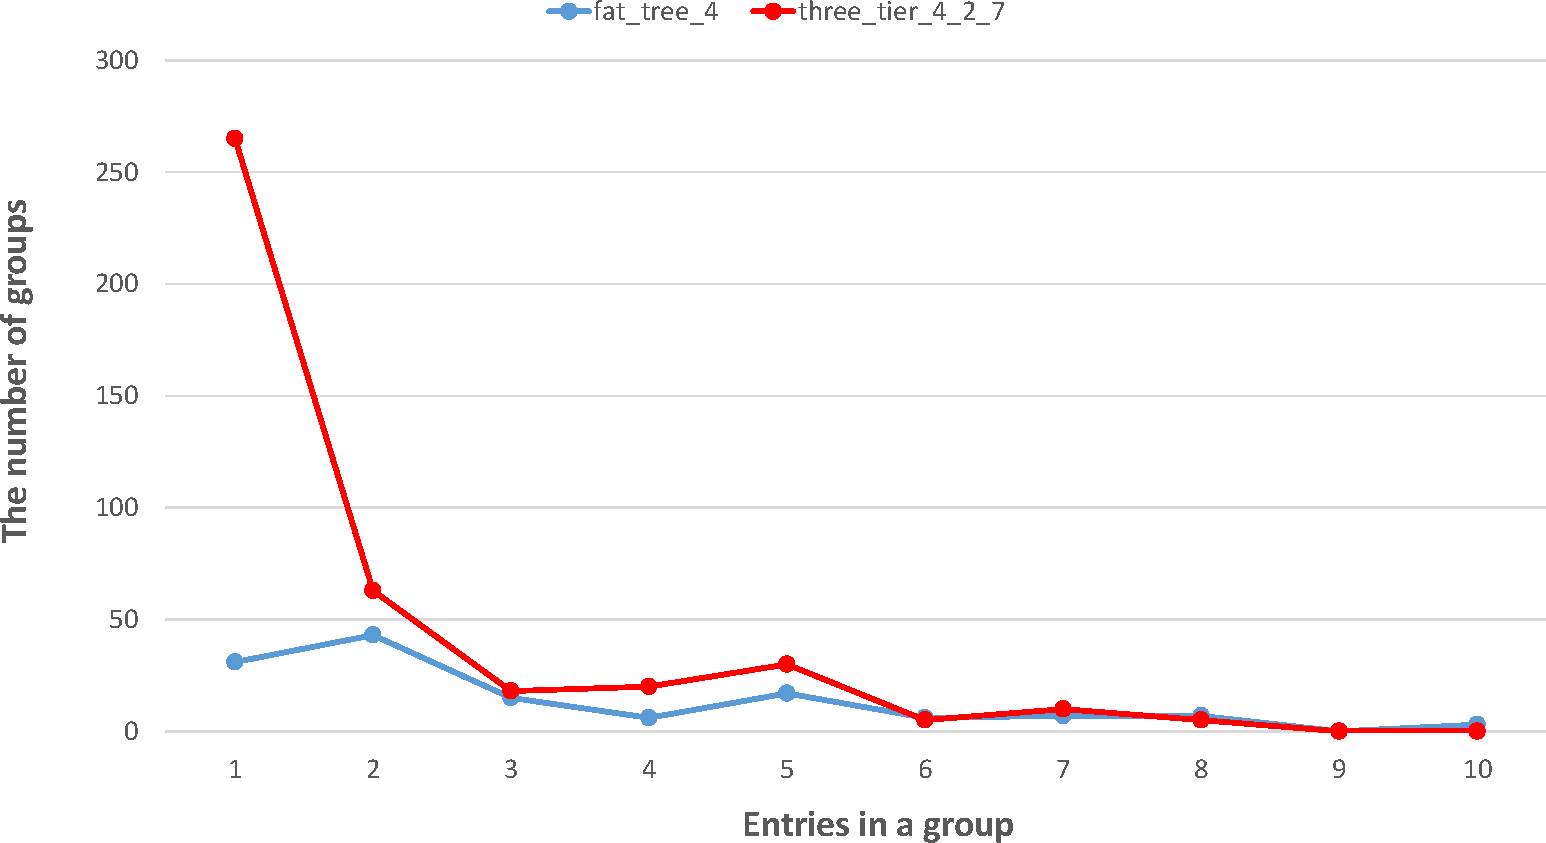
\includegraphics[width=1\linewidth]{figures/exp_topotype_distribute.pdf}
\caption{The comparison between fat\_tree\_4 and three\_tier\_4\_2\_7 -- the number of aggregated groups than contain various number of entries.}
\label{different_topo_distribute}
\end{figure}

\subsection{Influence of network scale}
To observe how effective our method is for various network scales, various sizes of fat-tree topology will be used. Fat-tree topologies are chosen for this experiment because the other two topology types have influence on the experimental result mostly by the way switches are connected. The parameter $n$ (i.e., the number of pods) ranges from 2 to 14. Since the network scale grows significantly with a larger number of pods, we consider at most 14 pods. There are also 20 entries on each switch. The results are shown in Table~\ref{table:different_scale}, and the trend chart of effective aggregation rates and actual aggregation rates are shown in Figure~\ref{different_scale_rate_trend}.

\begin{table}
\centering
\caption{Influence of various network scales}
\begin{tabular}{|p{1.8cm}|p{1cm}|p{1.3cm}|p{1.1cm}|p{1.3cm}|}
\hline topology name & Effective aggregation rate & Actual aggregation rate & Execution time(sec) & Number of auxiliary entries \\
\hline
\hline fat\_tree\_2 & 2.70 & 2.84 & 1.26 & 35 \\
\hline fat\_tree\_4 & 2.96 & 3.27 & 8.27 & 142 \\
\hline fat\_tree\_6 & 2.85 & 3.27 & 19.16 & 327 \\
\hline fat\_tree\_8 & 2.81 & 3.29 & 33.03 & 589 \\
\hline fat\_tree\_10 & 2.91 & 3.37 & 51.81 & 921 \\
\hline fat\_tree\_12 & 2.89 & 3.36 & 74.78 & 1334 \\
\hline fat\_tree\_14 & 2.79 & 3.29 & 102.56 & 1800 \\
\hline
\end{tabular}
\label{table:different_scale}
\end{table}

In the trend chart of effective and actual aggregation rates in Figure~\ref{different_scale_rate_trend}, the aggregation rates are similar in various sizes of topology except fat\_tree\_2 which has lower aggregation rates due to fewer number of switches and links, and the scale does not have any clear effect on the aggregation rates. Theoretically, there should be positive and negative factors that will influence the aggregation rates. A positive factor, for example, is a larger number of links, which help to raise the chance of adopting an entry into a group if the ratio between the number of forwarding ports and entries are balanced. Some examples of negative factors are more entries to be fit into aggregated groups and more hosts that will stop an aggregated group from extension. The result shows that these factors break even, and the effectiveness of our method will not drop with the increasing topology size.

\begin{figure}[ht]
\centering
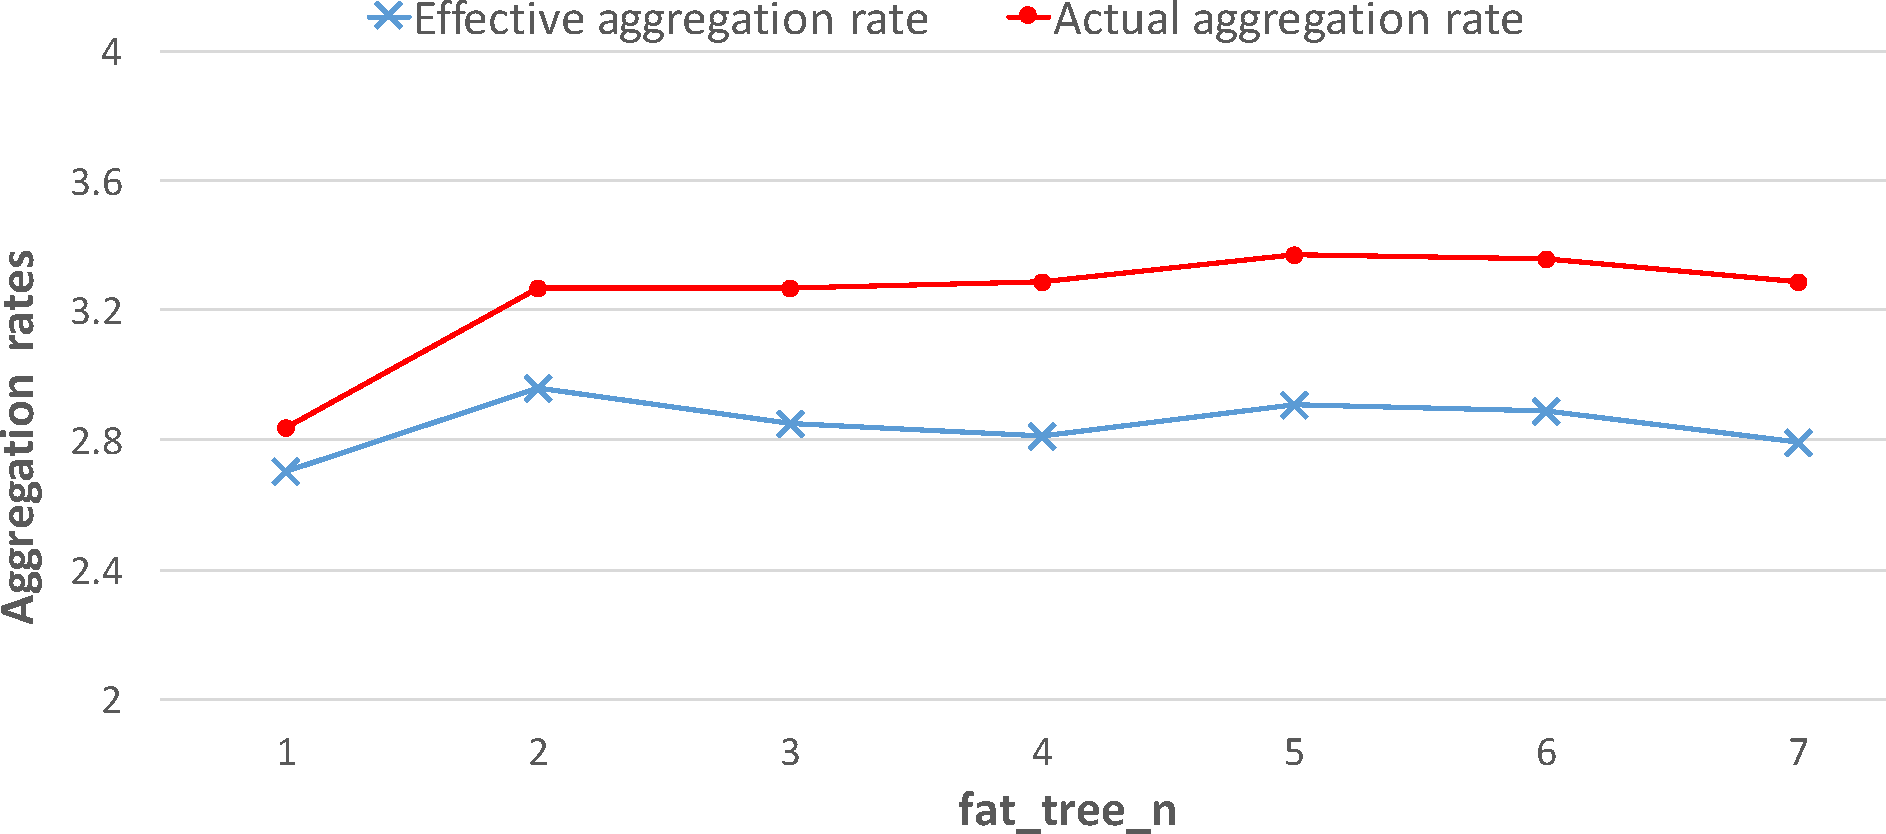
\includegraphics[width=1\linewidth]{figures/exp_scale_rate_trend.pdf}
\caption{The trend chart of aggregation rates under various scales of network.}
\label{different_scale_rate_trend}
\end{figure}

The relation between the topology size and the execution time are pretty similar, they are both proportional to $n^2$. It is quite as expected since the growth rate of switch is also proportional to $n^2$.

\subsection{Influence of flow entry number on each switch}
In this experiment, we will use only one topology -- fat\_tree\_4, and change the number of entries on each switch to see the influence it may bring. The number of entries on each switch increases from 10 to 200, and the intervals of entry number on each switch between every run increase as the number of entries on each switch grows, and the trend chart of effective aggregation rate with various number of entries on each switch is shown in Figure~\ref{exp_entrynum_trend}. The execution time and the number of auxiliary entries grow roughly linearly along with the number of entries on a switch.

\begin{table}
\centering
\caption{Aggregation rates, execution time and number of auxiliary entries for various number of entries on a switch.}
\begin{tabular}{|p{1.8cm}|p{1cm}|p{1.3cm}|p{1.1cm}|p{1.3cm}|}
\hline Number of entries per switch & Effective aggregation rate & Actual aggregation rate & Execution time (sec) & Number of auxiliary entry \\
\hline
\hline 10 & 2.38 & 3.15 & 3.98 & 72 \\
\hline 20 & 2.96 & 3.27 & 8.27 & 142 \\
\hline 30 & 3.01 & 3.64 & 15.03 & 214 \\
\hline 40 & 3.04 & 4.03 & 19.24 & 280 \\
\hline 50 & 3.18 & 4.22 & 26.19 & 346 \\
\hline 65 & 3.35 & 4.45 & 34.31 & 461 \\
\hline 80 & 3.41 & 4.51 & 41.47 & 560 \\
\hline 100 & 3.43 & 4.47 & 55.58 & 672 \\
\hline 120 & 3.48 & 4.45 & 64.96 & 812 \\
\hline 160 & 3.60 & 4.69 & 89.21 & 1070 \\
\hline 200 & 3.60 & 4.62 & 119.47 & 1359 \\
\hline 
\end{tabular}
\label{table:different_entry_per_switch}
\end{table}

\begin{figure}[ht]
\centering
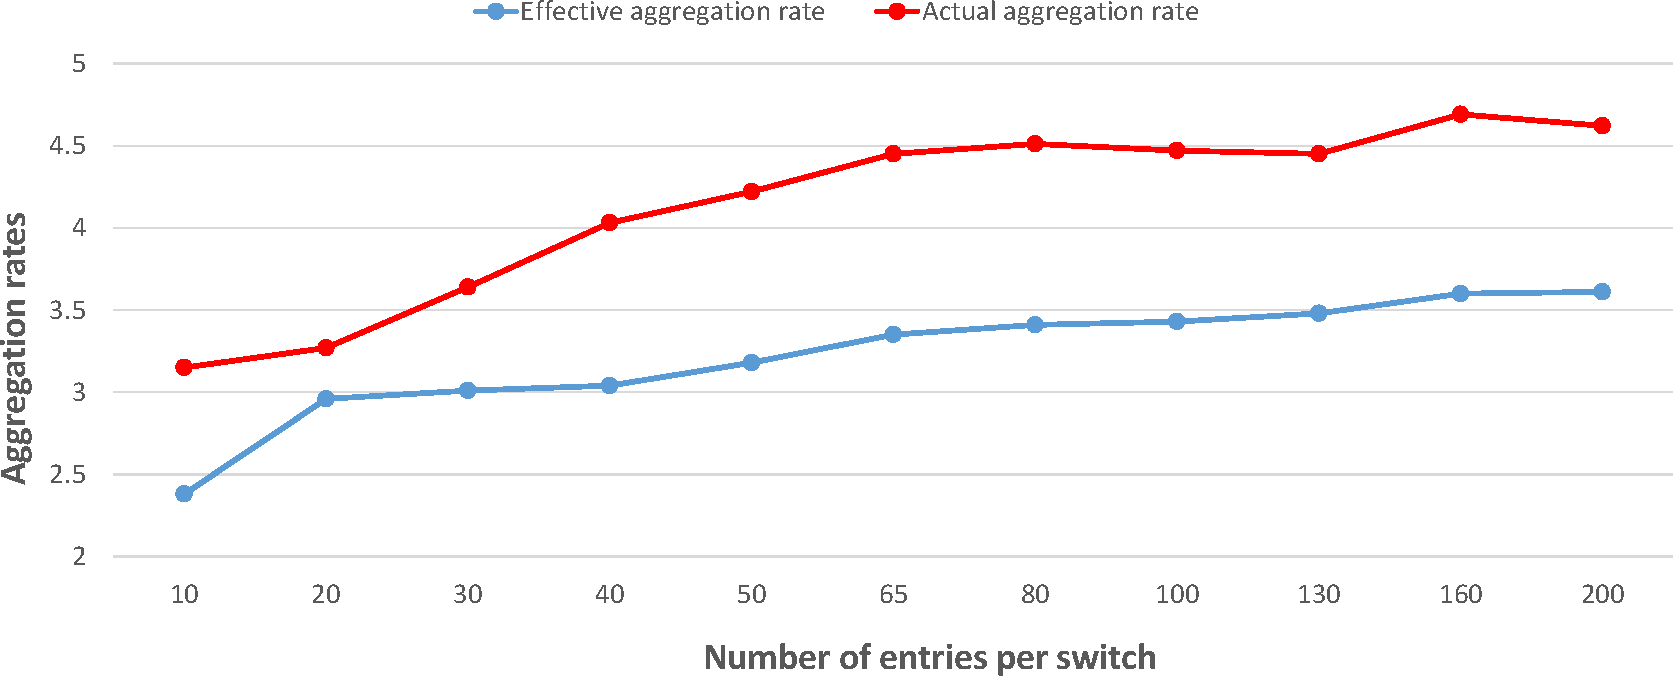
\includegraphics[width=1\linewidth]{figures/exp_entrynum_trend.pdf}
\caption{The trend chart of effective aggregation rate and actual aggregation rate with various number of entries per switch.}
\label{exp_entrynum_trend}
\end{figure}

From the trend chart in Figure~\ref{exp_entrynum_trend}, we can clearly see that the aggregation rates grow as the number of entries in the switch increases from 5 to 50 entries per switch. However, the growth rate decreases slowly after 50 entries per switch as the number of entries gets larger. A reasonable explanation for this phenomenon is the limited number of fields in a detection packet. Two fields can be selected at each L2/L3/L4 layer at most. For example, after entries with the match fields ``source IP'' and ``destination IP'', which are both at IP layer, are chosen into an aggregated group, it is impossible to add another entry whose match field is also at IP layer. Hence, a detection packet is able to accommodate no more than 6 fields and values. Since effective aggregation rate means the average number of entries in the aggregated groups, from this perspective, we may infer that the effective aggregation rate should converge at 6 if the number of entries on each switch gets really large. We refer to a packet with 6 fields and values set as a saturated packet.

\subsubsection{Examination and discussion}
\label{examination_and_discussion}

Before the experiment, we expect that the higher degree it is, the higher chance that we are able to extend an aggregated group more, which will result in higher aggregation rates. However, according to the result in Table~\ref{table:different_topo_type}, it seems that it is not always true, since the two-tier topologies have the highest average degree overall but has a moderate result. The fat-tree topology has the best result, while the three-tier topologies tend to have the worse result. After tracking down the entries inside the two-tier topologies, we discover that although the number of degrees is high, the ratio between the number of forwarding ports and the number of entries is imbalanced. The ports for forwarding to the neighbors are uniformly distributed among the entries, and they indicate the forwarding paths to choose while finding an aggregated group. There are not as many paths as we expect for an aggregated group to choose during entry selection, and thus the aggregation rates of two-tier topologies are lower than those of the fat-tree topology. 

To justify the inference that the effective aggregation rate may converge at 6 if the number of entries on each switch gets large, we also conducted another run of experiment with 1000 entries on each switch. Different from the inference, it results in an effective aggregation rate of 4.46 and an actual aggregation rate of 5.87. After further inspecting the content in aggregated groups, we discover that due to how the \texttt{tcp\_port} field is generated, there are many entries with TCP source or destination 80. When these entries are met during the group finding process, it is likely for two aggregated groups to end up in the same location once the two groups pass through the same switch during the finding process. As a detection packet gets closer to saturation, it will also make it harder for the corresponding aggregated group to find another entry that satisfies the aggregation conditions. Therefore, we did not have the best effective aggregation rate even with a large number of entries per switch. 

From the above experiments and analysis, we have the following conclusions. First, although the network scales are the same, the way how the switches are connected to each other leads to significant differences. Second, the network scale does not have clear influence on the efficiency of the detection method. Last but not the least, the more entries there are in the switches, the higher aggregation rates we are able to get; but as the average effective aggregation rate get closer and closer to 6, the aggregation rates grow slower and slower. We can conclude that the detection method is effective. Moreover, in our experimental environments, the structures are at most three tiers, which means in real-case network structures with more tiers, the method can be even more effective.  

\section{Conclusion}
\label{conclusion}
In this work, we discuss the hazard that a compromised switch in SDN may bring. We propose an effective way to scan through the entire network for disobedient forwarding behavior and evaluate it with various network topology types, scales and number of entries on each switch. The experimental result demonstrates that our method is effective in a network topology with balanced structure. The method detects through all the entries in topology ``fat\_tree\_4'' with around 135 packets, topology ``two\_tier\_10\_10'' with around 150 packets and topology ``three\_tier\_5\_5\_2'' with around 180 packets. Also, the scale of the network topology does not affect the efficiency significantly, and the effective aggregation rate grows to 3.48 in a fat-tree topology once there are 120 entries in each switch. 

In future work, more realistic factors should be taken into consideration, such as the collaboration of multiple compromised switches and the entries with multiple match fields and wildcard fields. Furthermore, the aggregated group finding method performs DFS without any estimation, and the core algorithm can be improved by adding heuristics. Also, as the new versions of OpenFlow are released, the method should be able to be optimized with the support of new features. For example, the auxiliary entries can be installed on the egress table once it is fully supported.

% conference papers do not normally have an appendix
% use section* for acknowledgment
%\section*{Acknowledgment}


%The authors would like to thank...

% trigger a \newpage just before the given reference
% number - used to balance the columns on the last page
% adjust value as needed - may need to be readjusted if
% the document is modified later
%\IEEEtriggeratref{8}
% The "triggered" command can be changed if desired:
%\IEEEtriggercmd{\enlargethispage{-5in}}

% references section

% can use a bibliography generated by BibTeX as a .bbl file
% BibTeX documentation can be easily obtained at:
% http://mirror.ctan.org/biblio/bibtex/contrib/doc/
% The IEEEtran BibTeX style support page is at:
% http://www.michaelshell.org/tex/ieeetran/bibtex/
%\bibliographystyle{IEEEtran}
% argument is your BibTeX string definitions and bibliography database(s)
%\bibliography{IEEEabrv,../bib/paper}
%
% <OR> manually copy in the resultant .bbl file
% set second argument of \begin to the number of references
% (used to reserve space for the reference number labels box)
\begin{thebibliography}{1}

\bibitem{OF_SPEC}
OpenFlow Switch Version 1.5 Specification, \url{https://www.opennetworking.org/images/stories/downloads/sdn-resources/onfspecifications/openflow/openflow-switch-v1.5.1.pdf}.

\bibitem{SOS13}
S. Scott-Hayward, G. O’Callaghan and S. Sezer,
``SDN Security: A Survey,'' In Proc. of IEEE SDN for Future Networks and Services (SDN4FNS), pp. 1–7., Nov. 2013.

\bibitem{HXWG15}
S. Hong, L. Xu, H. Wang and G. Gu,
``Poisoning Network Visibility in Software-Defined Networks: New Attacks and Countermeasures,''  In Proceedings of the 22th Annual Network and Distributed System Security Symposium (NDSS), Feb. 2015.

\bibitem{CKGL15}
P. W. Chi, C. T. Kuo, J. W. Guo and C. L. Lei,
``How to Detect a Compromised SDN Switch,'' In Proc. of the 1st IEEE Conference Network of Softwarization (NetSoft), pp. 1-6., Apr. 2015.

\bibitem{PJL16}
C. Pang, Y. Jiang and Q. Li,
``FADE: Detecting Forwarding Anomaly in Software-Defined Networks,'' In Proc. IEEE International Conference of Communications (ICC), May. 2016.

\bibitem{ZKVM12}
H. Zengyz, P. Kazemianyz, G. Varghese and N. McKeowny,
``Automatic Test Packet Generation,'' In Proc. of the 8th International Conference on Emerging Networking Experiments and Technologies (CoNEXT), Dec. 2012.

\bibitem{OVS_OFCTL}
OpenvSwitch Manual, \url{http://openvswitch.org/support/dist-docs/ovs-ofctl.8.txt}.

\bibitem{LAB14}
L. Schehlmann, A. Sebastian, and B. Harald, 
``Blessing or curse? Revisiting security aspects of Software-Defined Networking,'' In Proc. of 10th IEEE International Conference on Network and Service Management (CNSM), Nov. 2014.

\bibitem{KJK}
A. Khandelwal, N. Jain and S. Kamara,
``Attacking Data Center Networks from the Inside,'' \url{https://www.microsoft.com/en-us/research/wp-content/uploads/2016/02/dcn.pdf}.
 
\bibitem{AAS14}
M. Antikainen, T. Aura, and M. Särelä,
``Spook in Your Network: Attacking an SDN with a Compromised OpenFlow Switch,'' In Proc. of Nordic Conference on Secure IT System (NordSec), Oct. 2014.

\bibitem{ARDC14}
K. Agarwal, E. Rozner, C. Dixon, J. Carter,
``SDN traceroute: Tracing SDN Forwarding without Changing Network Behavior,'' In Proc. of the 3rd ACM Workshop on HotTopics in Software Defined Networking (HotSDN), Aug. 2014.

\bibitem{BCKK15}
R. Bifulco, H. Cui, G. O. Karame, F. Klaedtke,
``Fingerprinting software-defined networks,'' In Proc. of 2015 IEEE 23rd International Conference on Network Protocols (ICNP), Nov. 2015.

\bibitem{FNSS}
Topology Package In FNSS API Documentation, \url{http://fnss.github.io/doc/core/apidoc/fnss.functions.html#topologies-package}.

\bibitem{PACKETOUT}
Flowgrammable SDN OpenFlow Doumentation Message-Layer Section, \url{http://flowgrammable.org/sdn/openflow/message-layer/packetout/}.

\bibitem{PORT_FREQ}
Network Traffic Breakdown By Protocol Discussion On WhatPulse, \url{http://dkqnkzjkqr9h2.cloudfront.net/forums/showthread.php?tid=6987}.

\end{thebibliography}

\end{document}



\comment{start}

\begin{algorithm}[ht]
  \begin{algorithmic}[1]
  \algrestore{find_group}
    \Function{find\_one\_group}{switch$, packet$, $visited\_switch$, $visited\_entry$}
      \If{$switch < 0$} //it's a host
        \State \Return $packet$;
      \EndIf
      \State Add $switch$ to $visited\_switch$;
      \State $\textit{selected\_entry} \gets \Call{Get\_entry\_match\_packet}{\textit{switch}, \textit{packet}}$;
      \If{$selected\_entry$} // found an entry that current packet matches
        \State Add $selected\_entry$ to $visited\_entry$;
        
        \If{$selected\_entry$.$destination$ is a host}
          \State Add auxiliary entry that forward back to the controller;
          \State \Return $packet$;
        \Else
          \State Add $entry$ to $aggregated\_group$;
          \State \Call{find\_one\_group}{$destination$, $packet$, $visited\_switch$, $visited\_entry$}; //move on to next depth
        \EndIf
      \EndIf
  \algstore{find_group}
  \end{algorithmic}
\end{algorithm}

\begin{algorithm}[ht]
  \begin{algorithmic}[1]
  \algrestore{find_group}
      \State // no entry in this switch has the match field and value that packet matches;
      \State $\textit{output\_set} \gets empty$;  //  the output ports auxiliary entry out to
      \State $\textit{entry\_fit} \gets empty$; 
      \ForAll{$entry\;in\;switch$}
        \State $\textit{field, value, destination, cookie} \gets extract(\textit{entry})$;
        \If{$cookie$ not in $visited\_entry$ and $destination$ not in $visited\_switch$ and no entry with same field and value exist in $parent\_switch$ for all $\textit{parent\_switch} \in \textit{visited\_switch}$} 
          //  the entry fits the aggregation conditions
          \State Add $entry$ to $aggregated\_group$;
          \State $\textit{packet}[\textit{field}] \gets \textit{value}$;  //add match field to detection packet
          \State Add cookie of $selected\_entry$ to $visited\_entry$;
          \State Add output port to destination to $output\_set$
          \If{$destination$ is a host}
            \State Add an auxiliary entry on $switch$ with forwarding action back to the controller;
          \EndIf
          \State \Call{find\_one\_group}{$destination$, $packet$, $visited\_switch$, $visited\_entry$}; 
        \EndIf
      \EndFor
      \If{$output\_set$ has more than one element}
        \State $Add\;auxiliary\;entry\;on\;\textit{switch}\;with\;forwarding\;action\;to\;elements\;\in\;
        \textit{output\_set}$;
      \EndIf
      \State \Return $packet$;
    \EndFunction
\end{algorithmic}
\end{algorithm}
\comment{end}